\chapter{Advances}
\label{chap:advances}

\begin{figure}[hb]
\centering
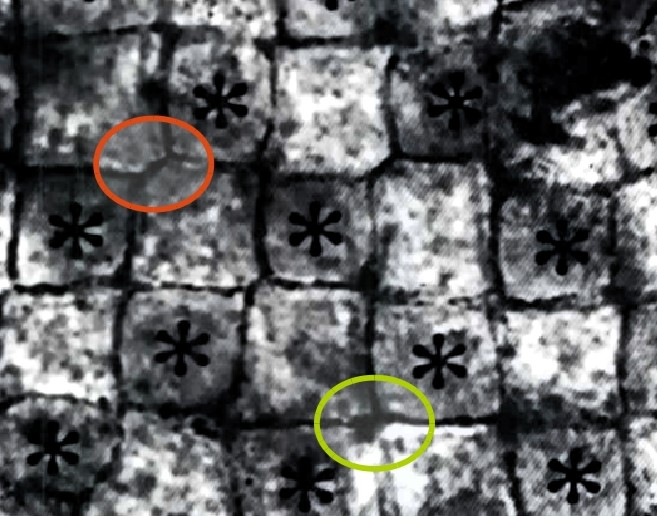
\includegraphics[width=0.5\textwidth]{../diagrams/checkers.jpg}
\caption{Square Cells in Quail Epithelium}
\end{figure}

An image or Japanese quail epithelium. This tissue is patterned like a checkerboard and has been modeled in the past as a tissue with degree three vertices. It is possible that modelling this tissue as degree four vertices would provide better approximations of the dynamics.  In particular, notice that the orange vertices clearly can be modeled with degree three, wherease the green vertex could be one degree four vertex or two degree three.\cite{Checkers}


What happens to the system if we change the vertices to degree 4? How will the equilibria compare?
Perhaps a new model force will becom apparent?

\section{Further Parallelization}
Data Redundancy

\section{A New Potential, A New Force}
Change the constant $\Beta$ to $\beta(P)$, a function of the perimeter. After differentiating, and using the chain rule, what can be said about the appearance of the new force?

\section{Images}
Imaging input initial condition

\section{Periodic Voronoi Mesh}
C++ doesnt have a bounding box algorithm for the voronoi mesh, or a periodic voronoi algorithm. These would be valuable contributions to the C++ Boost libraries. 

\section{Visualization SOftware }

That is standard, and a step above Geomview. 


